\subsection{Implementierung von HTTPS und SSO Prototyp}\label{subsec:implementierung-von-https}

Die aktualisierte Version von Collectiqo beinhaltet die Implementierung von HTTPS.
Die ursprüngliche Motivation hinter der Implementierung war, dass geplant war Single Sign On von Apple und Google einzubauen.
Beide dieser Unternehmen haben als Voraussetzung für die Implementierung ihrer jeweiligen Services, dass die Website HTTPS unterstützt.
Es wurden eigene Branches für die Programmierung an SSO eröffnet, in denen bereits erste Ansätze implementiert wurde.
Da der Branch auf einer alten Version von Collectiqo basiert, ist noch das alte Design in diesen Screenshots zu sehen.
Die SSO Implementierung sieht bisher wie folgt aus:

\begin{figure}[h]
    \centering
    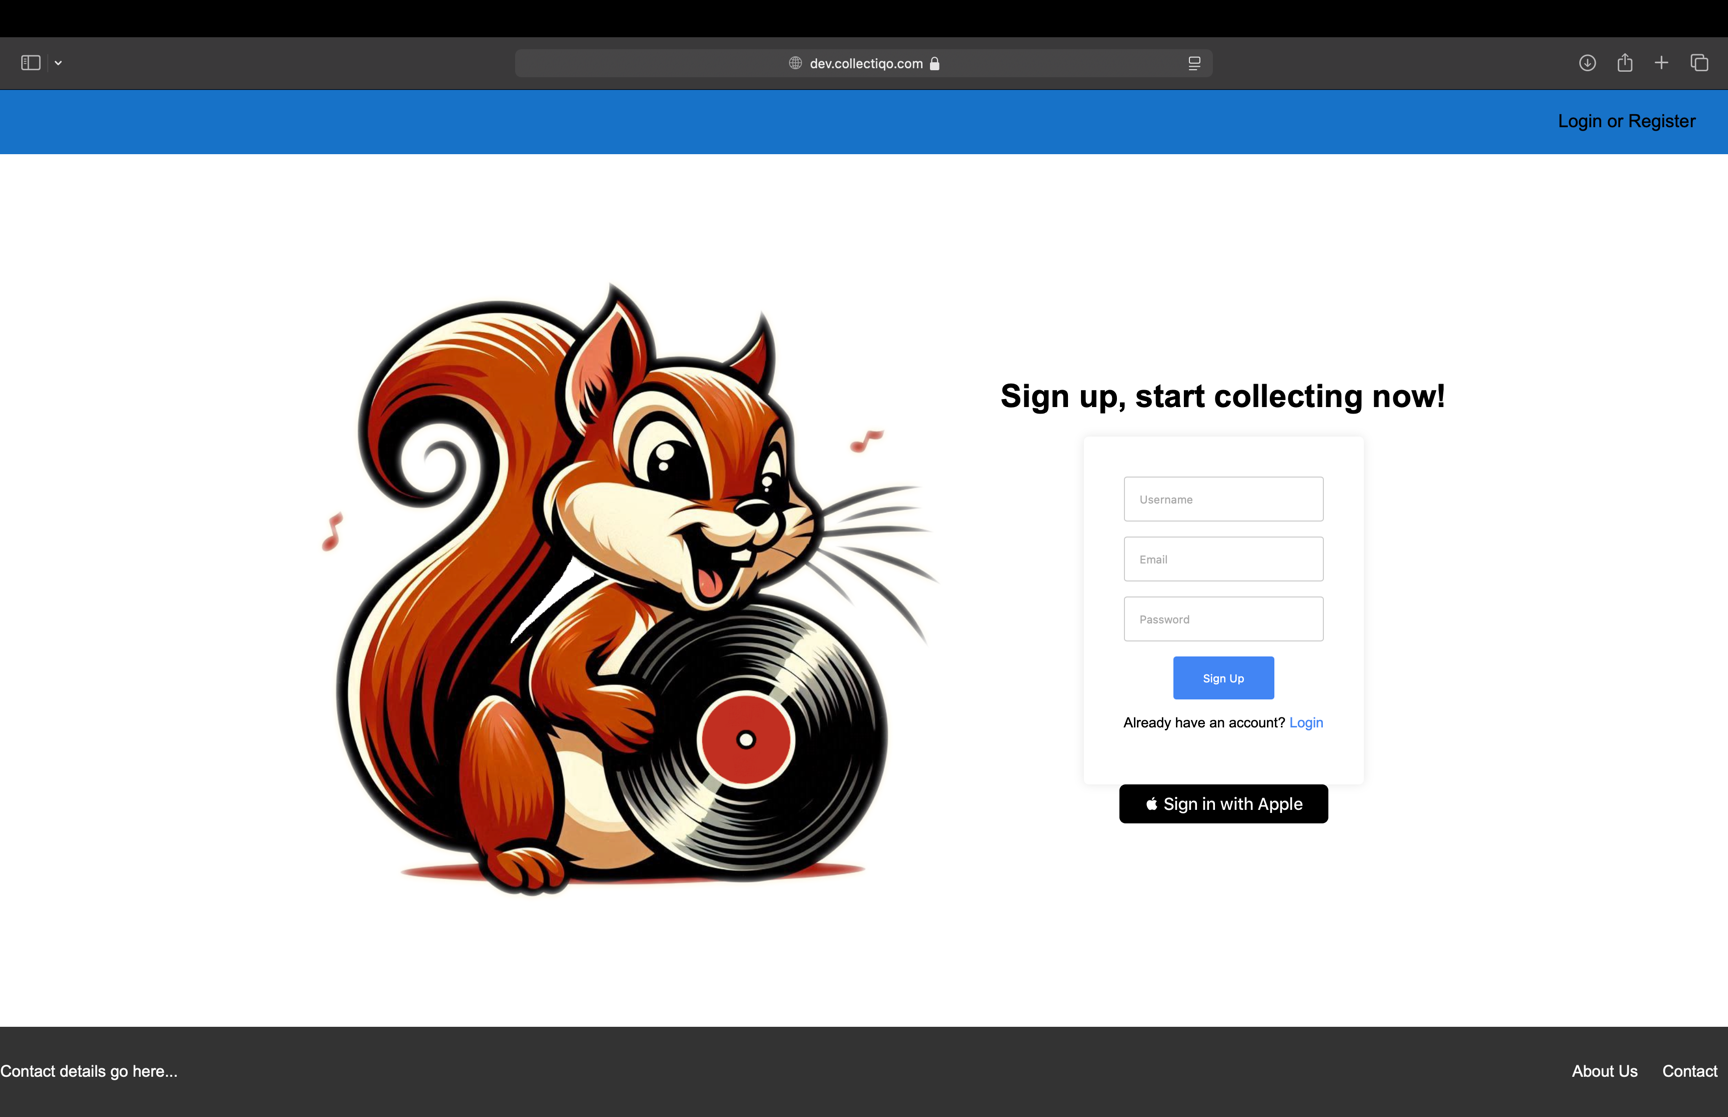
\includegraphics[width=0.7\textwidth]{apple_sso_1}
    \caption{Apple SSO 1}
    \label{fig:apple_sso_1}
\end{figure}

Beim Klicken des Buttons öffnet sich auch bereits das Apple Sign On Fenster:

\begin{figure}[h]
    \centering
    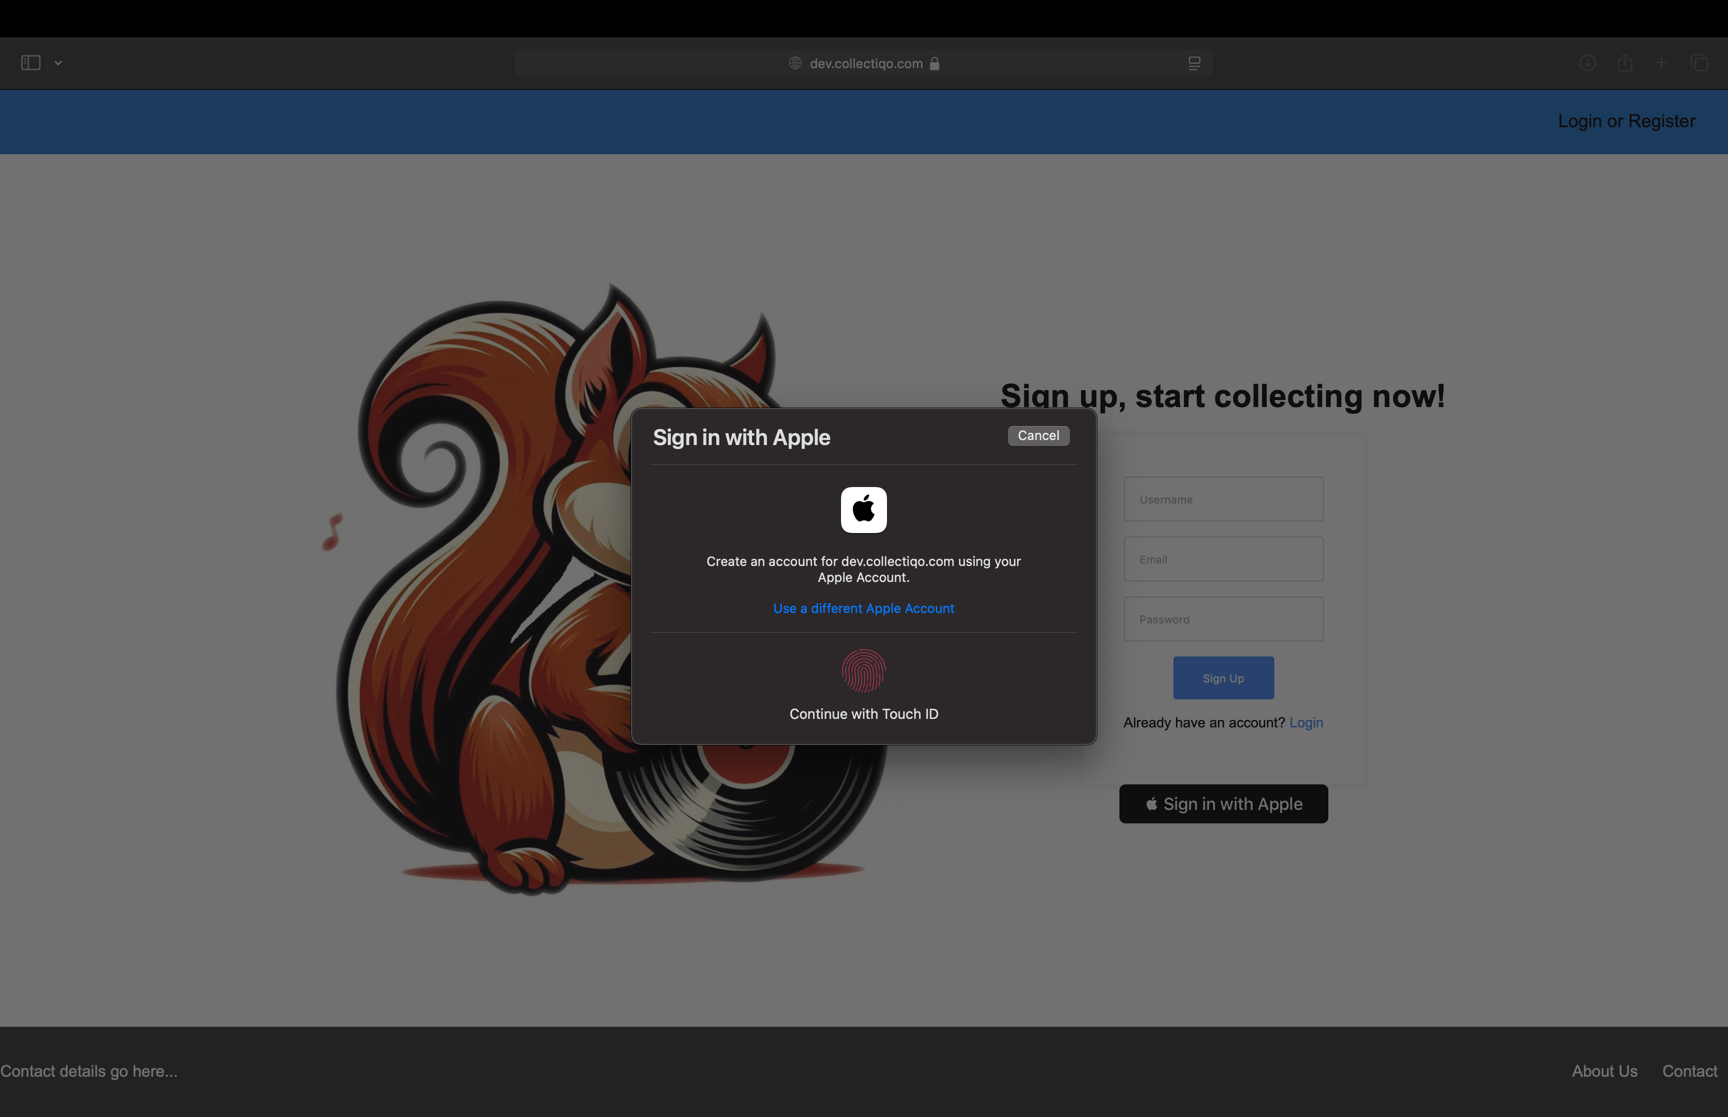
\includegraphics[width=0.7\textwidth]{apple_sso_2}
    \caption{Apple SSO 2}
    \label{fig:apple_sso_2}
\end{figure}

Grundlage dieses Prototyps war die Implementierung von HTTPS für die Website.
NodeJS besitzt eine eigene HTTPS Klassen, mit der das Programm gestartet werden kann:

\vspace{1em}
\lstset{language=JavaScript}
\begin{lstlisting}[label={lst:https}]
// starts app with https protocol
https.createServer(options, app).listen(port, () => {
    console.log(`App running on https://dev.collectiqo.com:${port}`);
});
\end{lstlisting}
\vspace{1em}

Voraussetzung für HTTPS ist ein Zertifikat, was mit einem Key gesigned wird.
Üblicherweise läuft diese Zertifizierung über eine Certificate Authority ab, welches für lokale Entwicklung über das Ziel hinaus schießt.
Für eine Entwicklungsumgebung reicht es aus, mit einem Self Signed Certificate zu arbeiten.
Hierbei wird ein lokaler Schlüssel generiert, sowie eine zertifikats Datei.
Diese beiden Dateien wurden auf den verschiedenen Entwicklungsmaschinen mit dem Tool OpenSSL erstellt.
Folgender Befehl wurde genutzt:

\vspace{1em}
\lstset{language=sh}
\begin{lstlisting}[label={lst:openssl}]
openssl req -newkey rsa:4096 -nodes -keyout local.key -x509 -days 365 -out local.crt -subj "/CN=dev.collectiqo.com" -addext "subjectAltName=DNS:dev.collectiqo.com"}
\end{lstlisting}
\vspace{1em}

Im Browser muss dann das Zertifikat als vertrauenswürdig eingetragen werden.
Im Befehl wird 'dev.collectiqo.com' als Domain für dieses Zertifikat hinterlegt, nur ist ohne weitere Konfiguration die App lokal nicht über diese Adresse erreichbar.
Damit die Domain lokal auf die korrekte IP-Adresse aufgelöst wird, muss die hostnames Datei angepasst werden.
Sind diese Vorbereitungen getroffen, so wird die Website vom Browser mit einer HTTPS Verbindung angezeigt:

\begin{figure}[h]
    \centering
    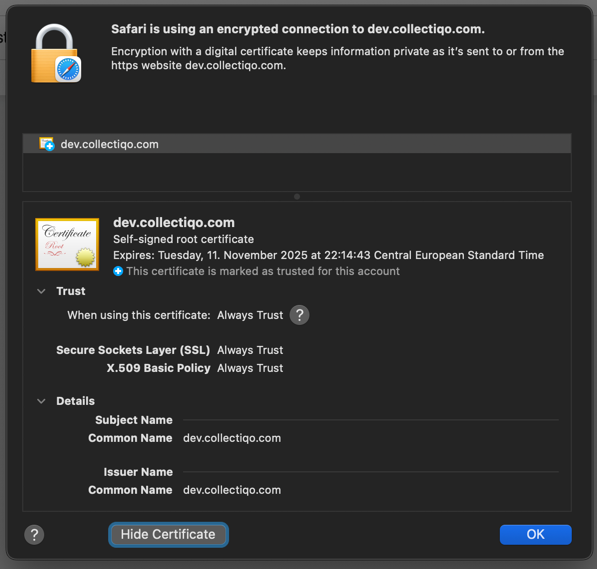
\includegraphics[width=0.5\textwidth]{https_browser}
    \caption{Zertifikat Ansicht in Safari}
    \label{fig:https_browser}
\end{figure}